% 第11章第6节：长度约束下的二次型极值（欧氏长度约束与Rayleigh商、加权长度约束与广义Rayleigh商、化归与广义特征方程、最优方向的核验与计算）。

\section{长度约束下的二次型极值}
\label{sec:ls-quadratic-extrema}

前五节建立了谱分解与奇异值分解，回答了线性作用在什么样的基下最简单。从本节开始，用这些分解解决三个具体问题，第一个是：固定实对称矩阵$\bm S$，输入方向改变时，二次型$\bm x^\top\bm S\bm x$最大、最小能取到多少，在哪些方向取到？

二次型随$\bm x$的长度按平方增长，不限制长度时只要把$\bm x$放大，数值就会跟着变，比较没有意义。所以先用欧氏长度约束$\bm x^\top\bm x=1$排除单纯缩放的影响，引入只依赖方向的Rayleigh商，并由谱分解求出它的极值。随后保持二次型不变，只改变规定单位长度的方式，得到广义Rayleigh商。通过坐标变换，加权长度约束可以化为普通的单位长度约束，由此导出广义特征方程及最优方向。下一节的最佳低秩逼近将直接使用本节的极值结论。

\subsection{欧氏长度约束与Rayleigh商}
\label{sec:ls-rayleigh-extremal}

先看最简单的对角矩阵$\bm S=\operatorname{diag}(4,1)$，此时$\bm x^\top\bm S\bm x=4x_1^2+x_2^2$。固定$\bm x^\top\bm x=1$，比较不同单位方向上的值：第一坐标方向$\bm e_1$给出$4$，第二坐标方向$\bm e_2$给出$1$。看起来最大值是$4$、最小值是$1$，但这只比较了两个候选。单位圆上还有无穷多个倾斜方向，例如$(1,1)^\top/\sqrt2$给出$5/2$；要证明全局极值，必须对所有单位方向都作出比较。长度约束在这里的作用是让比较只关注方向：若不加约束，把$\bm e_2$放大到$3\bm e_2$，二次型就变成$9$，超过了$\bm e_1$方向的值，这只反映了输入被放大，与方向无关。

把长度除掉，就得到只依赖方向的量，称为\term{Rayleigh商}（Rayleigh quotient）。
\begin{definition}[Rayleigh商]
\label{def:matrix-analysis-rayleigh-quotient}
对实对称矩阵$\bm S\in\mathbb R^{d\times d}$与$\bm x\neq\bm0$，
\begin{equation}
 R_{\bm S}(\bm x)=\frac{\bm x^\top\bm S\bm x}{\bm x^\top\bm x}.
 \label{eq:matrix-analysis-rayleigh-quotient}
\end{equation}
\end{definition}
把$\bm x$换成$c\bm x$（$c\neq0$）时分子分母同乘$c^2$，Rayleigh商不变，所以它只依赖$\bm x$所在的直线。对任意$\bm x\neq\bm0$，$R_{\bm S}(\bm x)$等于单位向量$\bm x/\lVert\bm x\rVert_2$上的二次型值；反过来，单位向量上的二次型值就是它的Rayleigh商。因此求Rayleigh商在全部非零向量上的极值，等价于在单位球面上求二次型的极值。

谱分解把这种比较化为对特征值的比较。按第~\ref{sec:ls-symmetric-spectral-decomposition}节的约定，把$\bm S$的特征值排成$\lambda_1\geq\cdots\geq\lambda_d$，对应标准正交特征向量$\bm q_1,\ldots,\bm q_d$。对单位向量$\bm x=\sum_ic_i\bm q_i$，有$\sum_ic_i^2=\lVert\bm x\rVert_2^2=1$，由二次型展开式~\eqref{eq:matrix-analysis-quadratic-spectral-form}，
\[
 R_{\bm S}(\bm x)=\sum_{i=1}^d\lambda_ic_i^2 .
\]
它是各特征值以$c_i^2$为权的加权平均：权重非负，总和为$1$。加权平均介于被平均各数的最小值与最大值之间，由此得到两端特征值的极值刻画。

\begin{theorem}[Rayleigh--Ritz]
\label{thm:matrix-analysis-rayleigh-ritz}
设$\bm S\in\mathbb R^{d\times d}$对称，特征值为$\lambda_1\geq\cdots\geq\lambda_d$，对应标准正交特征向量$\bm q_1,\ldots,\bm q_d$。则对一切$\bm x\neq\bm0$，
\begin{equation}
 \lambda_d\leq R_{\bm S}(\bm x)\leq\lambda_1 ,
 \label{eq:matrix-analysis-rayleigh-ritz}
\end{equation}
于是$\max_{\bm x\neq\bm0}R_{\bm S}(\bm x)=\lambda_1$，$\min_{\bm x\neq\bm0}R_{\bm S}(\bm x)=\lambda_d$，分别在$\bm q_1$与$\bm q_d$取到。进一步，$R_{\bm S}(\bm x)=\lambda_1$当且仅当$\bm x$是$\ker(\bm S-\lambda_1\bm I)$中的非零向量；$R_{\bm S}(\bm x)=\lambda_d$当且仅当$\bm x$是$\ker(\bm S-\lambda_d\bm I)$中的非零向量。
\end{theorem}
\begin{proof}
Rayleigh商不随缩放改变，只需对单位向量$\bm x=\sum_ic_i\bm q_i$证明。这时$R_{\bm S}(\bm x)=\sum_i\lambda_ic_i^2$且$\sum_ic_i^2=1$，所以
\[
 \lambda_1-R_{\bm S}(\bm x)=\sum_{i=1}^d(\lambda_1-\lambda_i)c_i^2\geq0 ,
\]
每一项都非负。同理$R_{\bm S}(\bm x)-\lambda_d=\sum_i(\lambda_i-\lambda_d)c_i^2\geq0$。这就是式~\eqref{eq:matrix-analysis-rayleigh-ritz}。取$\bm x=\bm q_1$时$c_1=1$、其余$c_i=0$，得$R_{\bm S}(\bm q_1)=\lambda_1$；取$\bm x=\bm q_d$得$\lambda_d$。所以两端的界都能取到。

再看取等条件。上面的和式等于零，当且仅当每一项都为零，即凡$\lambda_i<\lambda_1$的$i$都有$c_i=0$。这恰好说明$\bm x$落在满足$\lambda_i=\lambda_1$的那些$\bm q_i$的张成中；由定理~\ref{thm:ls-spectral-projections}，这个张成就是特征空间$\ker(\bm S-\lambda_1\bm I)$。最小值的情形相同。
\end{proof}

图~\ref{fig:ls-sphere-constrained-extremum}用一个二阶对称矩阵画出这一关系：二次型的水平椭圆在特征方向处与单位圆相切，切点处取到极值。

\begin{figure}[htbp]
  \centering
  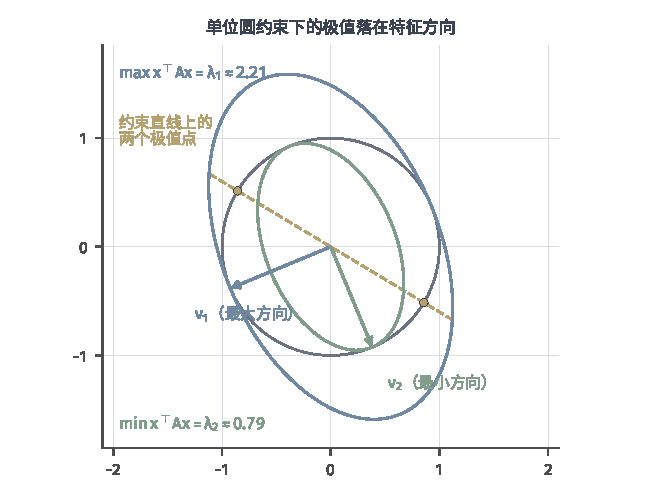
\includegraphics[width=112mm]{figures/00-shared/mathematical-preliminaries-upper/02-linear-spaces/matplotlib/ls-sphere-constrained-extremum/ls-sphere-constrained-extremum.pdf}
  \caption{单位圆约束下的极值落在特征方向。$\bm S=\left[\begin{smallmatrix}2&0.5\\0.5&1\end{smallmatrix}\right]$，
  灰圆为$\lVert\bm x\rVert=1$。蓝椭圆$\bm x^\top\bm S\bm x=\lambda_1\approx2.21$在
  $\pm\bm v_1$处与单位圆相切（最大值），绿椭圆$=\lambda_2\approx0.79$在$\pm\bm v_2$处
  相切（最小值）；黄色虚线为子空间约束直线，其上黄点是该约束下的两个极值，
  第~\ref{sec:ls-spectral-value-sensitivity}节的最小最大原理使用这种限制。
  $\lambda_{1,2}=(3\pm\sqrt2)/2$。固定复算。}
  \label{fig:ls-sphere-constrained-extremum}
\end{figure}

回到开头的例子，现在可以完成全部单位方向的比较。

\begin{example}[对角矩阵在全部单位方向上的比较]
\label{ex:ls-rayleigh-diagonal-two-by-two}
取$\bm S=\operatorname{diag}(4,1)$。每个单位向量都能写成$\bm x=(\cos\theta,\sin\theta)^\top$，其中$\theta\in[0,2\pi)$，于是
\[
 \bm x^\top\bm S\bm x=4\cos^2\theta+\sin^2\theta=1+3\cos^2\theta .
\]
由$0\leq\cos^2\theta\leq1$，它介于$1$与$4$之间：$\cos^2\theta=1$即$\bm x=\pm\bm e_1$时取最大值$4$，$\cos^2\theta=0$即$\bm x=\pm\bm e_2$时取最小值$1$。

结论：最大值$4$与最小值$1$正是两个特征值，取到它们的方向正是特征方向，与定理~\ref{thm:matrix-analysis-rayleigh-ritz}一致；倾斜方向的值都严格介于两者之间。
\end{example}

定理不要求$\bm S$半正定。二次型可以取负值，例如$\bm S=\operatorname{diag}(1,-2)$时$\bm x^\top\bm S\bm x=x_1^2-2x_2^2$，单位方向上的值仍介于$-2$与$1$之间，两端分别在$\pm\bm e_2$与$\pm\bm e_1$取到。

还要区分最优值与最优方向的唯一性。最大值$\lambda_1$总是唯一的数，取到它的方向则由特征空间$\ker(\bm S-\lambda_1\bm I)$决定。$\lambda_1$单重时，这个空间是一条直线，单位最优方向只有$\pm\bm q_1$两个，相差一个符号；$\lambda_1$重复时，空间中每个单位向量都给出最大值，例如$\bm S=\bm I$时所有单位方向都是最优的。重根时谱分解的$\bm q_1$只是其中一个代表，取决于特征基的选择，而最优方向组成的集合由定理~\ref{thm:ls-spectral-projections}唯一确定。最小值的情形相同。

一个常见的特例是$\bm S=\bm A^\top\bm A$，其中$\bm A\in\mathbb R^{m\times d}$。这时
\[
 R_{\bm A^\top\bm A}(\bm x)=\frac{\bm x^\top\bm A^\top\bm A\bm x}{\bm x^\top\bm x}=\frac{\lVert\bm A\bm x\rVert_2^2}{\lVert\bm x\rVert_2^2},
\]
即输出长度与输入长度之比的平方。第~\ref{sec:ls-svd}节已经说明$\bm A^\top\bm A$的特征值是奇异值的平方（$d>m$时补上零），所以定理~\ref{thm:matrix-analysis-rayleigh-ritz}给出那里最大、最小输出长度的另一种解释：单位输入的输出长度最大为$\sigma_1$，在$\bm v_1$取到；最小为$\sqrt{\lambda_d}$，其中$\lambda_d$是$\bm A^\top\bm A$的最小特征值，在它的特征方向取到。第~\ref{sec:linear-algebra-homogeneous-estimation}节的齐次最小二乘正是在单位输入中最小化这一量：若$\bm A$有非零的零空间，最小值为零，任一单位零空间向量都最优；若$\bm A$满列秩，则$\bm A\bm x\neq\bm0$对一切$\bm x\neq\bm0$成立，$\bm A^\top\bm A\succ0$，由定理~\ref{thm:ls-symmetric-definiteness-eigenvalues}，最小值为正。第~\ref{sec:ls-low-rank-approximation}节将从重建误差出发，引出另一个用Rayleigh商求解的问题。

\subsection{加权长度约束与广义Rayleigh商}
\label{sec:ls-generalized-rayleigh}

上一小节用欧氏长度规定“单位输入”。各坐标的单位或重要性不同时，长度往往按第~\ref{sec:ls-weighted-inner-products}节的加权内积度量，约束也随之改变。保持$\bm S=\operatorname{diag}(4,1)$不变，改用$\bm B=\operatorname{diag}(9,1)$，规定$\bm x^\top\bm B\bm x=9x_1^2+x_2^2=1$。沿第一坐标方向，满足约束的向量是$\pm\bm e_1/3$，二次型值为$4\cdot(1/3)^2=4/9$；沿第二坐标方向，满足约束的向量仍是$\pm\bm e_2$，值为$1$。在欧氏约束下最优的$\bm e_1$方向，现在不如$\bm e_2$方向。可见改变长度标准会改变答案；而且与上一小节一样，比较两个坐标方向还不够，必须比较全部满足加权约束的方向。

与欧氏情形相同，先把约束化为一个不随缩放改变的商。
\begin{definition}[广义Rayleigh商]
\label{def:ls-generalized-rayleigh-quotient}
设$\bm S\in\mathbb R^{d\times d}$对称，$\bm B\in\mathbb R^{d\times d}$对称正定。对$\bm x\neq\bm0$，称
\begin{equation}
 R_{\bm S,\bm B}(\bm x)=\frac{\bm x^\top\bm S\bm x}{\bm x^\top\bm B\bm x}
 \label{eq:ls-generalized-rayleigh-quotient}
\end{equation}
为$\bm S$关于$\bm B$的\term{广义Rayleigh商}（generalized Rayleigh quotient）。
\end{definition}
$\bm B$正定保证分母$\bm x^\top\bm B\bm x$对一切$\bm x\neq\bm0$为正，商有定义。把$\bm x$换成$c\bm x$（$c\neq0$）时分子分母同乘$c^2$，商不变。对任意$\bm x\neq\bm0$，令$\bm u=\bm x/\sqrt{\bm x^\top\bm B\bm x}$，则$\bm u^\top\bm B\bm u=1$且$R_{\bm S,\bm B}(\bm x)=\bm u^\top\bm S\bm u$；反过来，约束$\bm x^\top\bm B\bm x=1$上的二次型值就是广义Rayleigh商。所以求广义Rayleigh商的极值，等价于在$\bm x^\top\bm B\bm x=1$上比较$\bm x^\top\bm S\bm x$。

$\bm B=\bm I$时，广义Rayleigh商恰好回到普通Rayleigh商。两者比较的是同一个二次型$\bm x^\top\bm S\bm x$，差别只在于用哪种长度规定“单位输入”：普通Rayleigh商用欧氏长度，广义Rayleigh商用加权长度$\lVert\bm x\rVert_{\bm B}$。

\subsection{化归与广义特征方程}
\label{sec:ls-generalized-eigen-reduction}

加权约束$\bm x^\top\bm B\bm x=1$的困难在于它不是欧氏单位球面，第~\ref{sec:ls-rayleigh-extremal}节的结论不能直接使用。思路是换一个坐标，使加权长度在新坐标中成为欧氏长度。由定理~\ref{thm:ls-gram-factor}，正定的$\bm B$可以写成$\bm B=\bm L^\top\bm L$，其中$\bm L$可逆。令$\bm z=\bm L\bm x$，则$\bm x=\bm L^{-1}\bm z$，且$\bm x\neq\bm0$当且仅当$\bm z\neq\bm0$。代入得
\[
 \bm x^\top\bm B\bm x=(\bm L\bm x)^\top(\bm L\bm x)=\bm z^\top\bm z,\qquad
 \bm x^\top\bm S\bm x=\bm z^\top\bm L^{-\top}\bm S\bm L^{-1}\bm z ,
\]
其中$\bm L^{-\top}$表示$(\bm L^{-1})^\top$。记
\[
 \bm C=\bm L^{-\top}\bm S\bm L^{-1},
\]
则$\bm C^\top=\bm L^{-\top}\bm S^\top\bm L^{-1}=\bm C$，仍是实对称矩阵，而
\[
 R_{\bm S,\bm B}(\bm x)=\frac{\bm z^\top\bm C\bm z}{\bm z^\top\bm z}=R_{\bm C}(\bm L\bm x).
\]
加权约束问题就化成了$\bm C$的普通Rayleigh商问题，可以直接应用定理~\ref{thm:matrix-analysis-rayleigh-ritz}。这一化归只用到Gram因子与换元，不需要矩阵平方根、多元微分或Lagrange乘子法。

最优方向要从新坐标换回原坐标。若$\bm C\bm z=\mu\bm z$，令$\bm v=\bm L^{-1}\bm z$，则$\bm L^{-\top}\bm S\bm v=\mu\bm L\bm v$，两边左乘$\bm L^\top$得
\[
 \bm S\bm v=\mu\bm L^\top\bm L\bm v=\mu\bm B\bm v .
\]
反过来，若$\bm S\bm v=\mu\bm B\bm v$且$\bm v\neq\bm0$，左乘$\bm L^{-\top}$并令$\bm z=\bm L\bm v$，就得到$\bm C\bm z=\mu\bm z$。所以，$\bm C$的特征对与下面方程的解一一对应。

\begin{definition}[广义特征值]
\label{def:matrix-analysis-generalized-eigenvalue}
对实对称$\bm S$与对称正定$\bm B$，称满足
\begin{equation}
\begin{gathered}
\bm S\bm v=\mu\bm B\bm v\\
\bm v\neq\bm0
\end{gathered}
\label{eq:matrix-analysis-generalized-eigenproblem}
\end{equation}
的$\mu$为广义特征值，$\bm v$为属于$\mu$的广义特征向量，求解它们的问题称为\term{广义特征问题}（generalized eigenvalue problem）。
\end{definition}

广义特征值不依赖Gram因子$\bm L$的选取。由$\bm S-\mu\bm B=\bm L^\top(\bm C-\mu\bm I)\bm L$，
\[
 \det(\bm S-\mu\bm B)=(\det\bm L)^2\det(\bm C-\mu\bm I),
\]
而$\det\bm L\neq0$，所以广义特征值恰是$\det(\bm S-\mu\bm B)=0$的根，也就是$\bm C$的特征值；不同的$\bm L$给出不同的$\bm C$，特征值却相同。$\bm C$对称，由谱定理，这些根全是实数，按重数计共有$d$个，下面记为$\mu_1\geq\cdots\geq\mu_d$。把定理~\ref{thm:matrix-analysis-rayleigh-ritz}用于$\bm C$并换回原坐标，就得到加权约束问题的解。

\begin{theorem}[广义Rayleigh商的极值]
\label{thm:ls-generalized-rayleigh-extremal}
设$\bm S$对称、$\bm B$对称正定，广义特征值为$\mu_1\geq\cdots\geq\mu_d$。则对一切$\bm x\neq\bm0$，
\[
 \mu_d\leq R_{\bm S,\bm B}(\bm x)\leq\mu_1 .
\]
$R_{\bm S,\bm B}(\bm x)=\mu_1$当且仅当$\bm S\bm x=\mu_1\bm B\bm x$，$R_{\bm S,\bm B}(\bm x)=\mu_d$当且仅当$\bm S\bm x=\mu_d\bm B\bm x$。因此，在约束$\bm x^\top\bm B\bm x=1$上，$\bm x^\top\bm S\bm x$的最大值为$\mu_1$，最优解是满足$\bm v^\top\bm B\bm v=1$的属于$\mu_1$的广义特征向量；最小值的情形相同。
\end{theorem}
\begin{proof}
取$\bm B=\bm L^\top\bm L$与$\bm C=\bm L^{-\top}\bm S\bm L^{-1}$如上。$\bm C$的特征值就是$\mu_1\geq\cdots\geq\mu_d$。对$\bm x\neq\bm0$，令$\bm z=\bm L\bm x\neq\bm0$，由$R_{\bm S,\bm B}(\bm x)=R_{\bm C}(\bm z)$及定理~\ref{thm:matrix-analysis-rayleigh-ritz}，得$\mu_d\leq R_{\bm S,\bm B}(\bm x)\leq\mu_1$。

同一定理还说明，$R_{\bm C}(\bm z)=\mu_1$当且仅当$\bm C\bm z=\mu_1\bm z$。由上面的一一对应，这又当且仅当$\bm S\bm x=\mu_1\bm B\bm x$。$\bm C$确有属于$\mu_1$的特征向量，所以上界能够取到。最小值同理。

最后，约束$\bm x^\top\bm B\bm x=1$上的二次型值就是广义Rayleigh商，所以它的最大值为$\mu_1$，且只在满足$\bm S\bm x=\mu_1\bm B\bm x$与$\bm x^\top\bm B\bm x=1$的$\bm x$处取到。
\end{proof}

上面只用到$\bm C$两端的特征向量。对$\bm C$应用完整的谱分解，还能得到全部广义特征向量的结构：它们可以选得关于加权内积$\langle\cdot,\cdot\rangle_{\bm B}$互相正交。

\begin{theorem}[$\bm B$正交的广义特征向量]
\label{thm:ls-generalized-eigen-b-orthogonal}
设$\bm S$对称、$\bm B$对称正定，广义特征值为$\mu_1\geq\cdots\geq\mu_d$。则存在$\bm v_1,\ldots,\bm v_d$，使
\[
 \bm S\bm v_i=\mu_i\bm B\bm v_i,\qquad \bm v_i^\top\bm B\bm v_j=\delta_{i,j}\quad(i,j=1,\ldots,d).
\]
记$\bm V=[\bm v_1,\ldots,\bm v_d]$，$\bm M=\operatorname{diag}(\mu_1,\ldots,\mu_d)$，上式等价于$\bm V^\top\bm B\bm V=\bm I$与$\bm V^\top\bm S\bm V=\bm M$。
\end{theorem}
\begin{proof}
由谱定理，$\bm C=\bm Z\bm M\bm Z^\top$，其中$\bm Z=[\bm z_1,\ldots,\bm z_d]$为正交矩阵，$\bm C\bm z_i=\mu_i\bm z_i$。令$\bm V=\bm L^{-1}\bm Z$，即$\bm v_i=\bm L^{-1}\bm z_i$。由上面的一一对应，$\bm S\bm v_i=\mu_i\bm B\bm v_i$。又
\[
\begin{gathered}
 \bm V^\top\bm B\bm V=\bm Z^\top\bm L^{-\top}\bm L^\top\bm L\bm L^{-1}\bm Z=\bm Z^\top\bm Z=\bm I,\\
 \bm V^\top\bm S\bm V=\bm Z^\top\bm L^{-\top}\bm S\bm L^{-1}\bm Z=\bm Z^\top\bm C\bm Z=\bm M .
\end{gathered}
\]
逐元素比较第一式即得$\bm v_i^\top\bm B\bm v_j=\delta_{i,j}$。
\end{proof}

$\bm V$可逆，所以任意$\bm x$都能写成$\bm x=\sum_ia_i\bm v_i$。由定理，$\bm x^\top\bm B\bm x=\sum_ia_i^2$，$\bm x^\top\bm S\bm x=\sum_i\mu_ia_i^2$，广义Rayleigh商再次成为特征值的加权平均，这与普通情形完全平行，只是坐标改成了$\bm B$正交的广义特征向量。至此两端极值都已求出。若还需要刻画中间的广义特征值，可以对$\bm C$使用第~\ref{sec:ls-spectral-value-sensitivity}节的Courant--Fischer最小最大原理（定理~\ref{thm:matrix-analysis-courant-fischer}），再按$\bm z=\bm L\bm x$换回原坐标。

\subsection{最优方向的核验与计算}
\label{sec:ls-generalized-eigen-check}

上一小节的定理给出了解的形式，这里回到二维例子，按化归的步骤算出最优方向，并核验它们确实满足约束与广义特征方程。

\begin{example}[加权约束下的最优方向]
\label{ex:ls-generalized-rayleigh-diagonal}
给定$\bm S=\operatorname{diag}(4,1)$与$\bm B=\operatorname{diag}(9,1)$，在$\bm x^\top\bm B\bm x=1$上求$\bm x^\top\bm S\bm x$的最大值、最小值与最优方向。

化归：取$\bm L=\operatorname{diag}(3,1)$，则$\bm L^\top\bm L=\bm B$，
\[
 \bm C=\bm L^{-\top}\bm S\bm L^{-1}=\operatorname{diag}\Bigl(\frac49,1\Bigr).
\]
由定理~\ref{thm:matrix-analysis-rayleigh-ritz}，$R_{\bm C}$的最大值为$1$，在$\bm z=\pm\bm e_2$取到；最小值为$4/9$，在$\bm z=\pm\bm e_1$取到。换回原坐标$\bm v=\bm L^{-1}\bm z$，最大方向为$\pm\bm e_2$，最小方向为$\pm\bm e_1/3$。

核验：$\bm e_2^\top\bm B\bm e_2=1$，$(\bm e_1/3)^\top\bm B(\bm e_1/3)=9/9=1$，两者都满足加权单位约束。又$\bm S\bm e_2=\bm e_2=1\cdot\bm B\bm e_2$，而
\[
 \bm S\frac{\bm e_1}{3}=\frac43\bm e_1=\frac49\cdot\bm B\frac{\bm e_1}{3},
\]
所以它们分别是属于$1$与$4/9$的广义特征向量，且$\bm e_2^\top\bm B(\bm e_1/3)=0$，满足$\bm B$正交。

直接比较全部可行方向：约束给出$x_2^2=1-9x_1^2$，其中$x_1^2\in[0,1/9]$，于是
\[
 \bm x^\top\bm S\bm x=4x_1^2+1-9x_1^2=1-5x_1^2\in\Bigl[\frac49,1\Bigr].
\]

结论：最大值为$1$，最优方向为$\pm\bm e_2$；最小值为$4/9$，最优方向为$\pm\bm e_1/3$。直接比较与化归结果一致，完成了全部可行方向的比较。
\end{example}

上面的例子中$\bm L$是对角矩阵，可以直接求逆。一般情形下，计算时也按化归的步骤进行，但通过因子分解与线性求解完成换元，不必显式形成$\bm L^{-1}$。第~\ref{chap:linear-equations-and-optimization}章的Cholesky分解把$\bm L$取成三角矩阵，于是$\bm C$可以分两步得到：先解三角方程组$\bm L^\top\bm W=\bm S$，得到$\bm W=\bm L^{-\top}\bm S$；再解$\bm L^\top\bm C^\top=\bm W^\top$，得到$\bm C=\bm W\bm L^{-1}$。求出$\bm C$的特征向量$\bm z$后，解三角方程组$\bm L\bm v=\bm z$换回原坐标。整个过程保持对称结构，只需对称矩阵的特征值算法。

另一种看似直接的做法是把$\bm S\bm v=\mu\bm B\bm v$左乘$\bm B^{-1}$，改求普通特征问题$\bm B^{-1}\bm S\bm v=\mu\bm v$。由$\bm B^{-1}\bm S=\bm L^{-1}\bm L^{-\top}\bm S=\bm L^{-1}\bm C\bm L$，它与$\bm C$相似，特征值相同；但$\bm B^{-1}\bm S$一般不对称。例如$\bm S=\left[\begin{smallmatrix}2&1\\1&2\end{smallmatrix}\right]$、$\bm B=\operatorname{diag}(2,1)$时，$\bm B^{-1}\bm S=\left[\begin{smallmatrix}1&1/2\\1&2\end{smallmatrix}\right]$。它的特征多项式为$z^2-3z+\tfrac32$，特征值为$\mu_{1,2}=(3\pm\sqrt3)/2$；由第一行$(1-\mu)x_1+\tfrac12x_2=0$得特征向量$\bm v_1=(1,1+\sqrt3)^\top$、$\bm v_2=(1,1-\sqrt3)^\top$。这两个向量就是广义特征向量，满足$\bm v_1^\top\bm B\bm v_2=2+(1-3)=0$，关于$\bm B$正交；但$\bm v_1^\top\bm v_2=1+(1-3)=-1\neq0$，在欧氏内积下并不正交。所以不能对$\bm B^{-1}\bm S$套用谱定理与欧氏正交特征基的结论。上面二维例子里$\bm B^{-1}\bm S$恰好是对角矩阵，只是一个特殊情形。

本节的化归依赖$\bm B$正定。若$\bm B$不是正定矩阵，$\bm x^\top\bm B\bm x$不再定义长度：$\bm B$半正定而奇异时，存在$\bm x\neq\bm0$使分母为零；$\bm B$不定时，$\bm x^\top\bm B\bm x$可以为负。这时也不存在可逆的$\bm L$使$\bm B=\bm L^\top\bm L$：若有这样的$\bm L$，则$\bm x\neq\bm0$时$\bm L\bm x\neq\bm0$，$\bm x^\top\bm B\bm x=\lVert\bm L\bm x\rVert_2^2>0$，$\bm B$就是正定的。于是化归无从进行，约束问题甚至可能没有极值。例如$\bm S=\bm I$、$\bm B=\operatorname{diag}(1,0)$时，约束$x_1^2=1$不限制$x_2$，而$\bm x^\top\bm S\bm x=1+x_2^2$没有上界。这类更一般的广义特征问题不在此展开。

本节由谱分解得到了长度约束下二次型的全部两端极值：欧氏约束下是$\bm S$的最大、最小特征值，加权约束下是最大、最小广义特征值，最优方向分别是相应的特征向量与广义特征向量。下一节的最佳低秩逼近把重建误差化为保留量的极大化，首先用到的就是这里的Rayleigh商结论。
